%To compile as handout, use
%pdflatex "\def\ishandout{1} \input{filename.tex}"
%Defaults to non-handout mode (with slide reveals)
\ifdefined\ishandout
  \documentclass[handout]{beamer}
\else
  \documentclass{beamer}
\fi
 
\usepackage{econ103slides} 

\date{Lecture 18}


\begin{document} 




%%%%%%%%%%%%%%%%%%%%%%%%%%%%%%%%%%%%%%%%

\begin{frame}[plain]
	\titlepage 
	

\end{frame} 



%%%%%%%%%%%%%%%%%%%%%%%%%%%%%%%%%%%%%%%%
\begin{frame}
\begin{center}
\Huge Confidence Intervals IV
\end{center}
\end{frame}

\begin{frame}
\frametitle{Confidence Interval ``Roundup''}

\begin{enumerate}
	\item Values near the middle of a CI are ``more plausible.''
	\item CI for Difference of Means using the CLT
	%\vspace{0.2in}
	\item Independent Samples versus Matched Pairs
	%\item Refined CIs for Population Proportion
	%\item Percentile Bootstrap CIs
\end{enumerate}

\alert{Note that we are no longer assuming that the population is normal. Instead, we are constructing confidence intervals based on a large sample approximation using the CLT.}

\end{frame}

%%%%%%%%%%%%%%%%%%%%%%%%%%%%%%%%%%%%%%%%
\begin{frame}
\frametitle{Are Republicans Better Informed Than Democrats?}
\framesubtitle{\fbox{\href{http://www.people-press.org/files/2012/08/8-10-12-Knowledge-release.pdf}{Pew: ``What Voters Know About Campaign 2012''}}}
Of the 239 Republicans surveyed, 47\% correctly identified John Roberts as the current chief justice. Only 31\% of the 238 Democrats surveyed correctly identified him. Is this difference meaningful or just sampling variation?

\vspace{2em}
\alert{Again, assume random sampling.}


%Might be better to make a confidence interval for the proportion MINUS 0.25 to account for random guessing.

\end{frame}
%%%%%%%%%%%%%%%%%%%%%%%%%%%%%%%%%%%%%%%%
\begin{frame}
\frametitle{Confidence Interval for a Difference of Proportions}
	\begin{block}{What is the appropriate probability model for the sample?} 
$X_1, \hdots, X_n \sim \mbox{ iid Bernoulli}(p)$ independently  of $Y_1, \hdots, Y_m \sim \mbox{ iid Bernoulli}(q)$
\end{block}
	\begin{block}{What is the parameter of interest?}
The difference of population proportions $p - q$
\end{block}

\begin{block}{What is our estimator?}
The difference of sample proportions: $\widehat{p} - \widehat{q}$ where:
	$$\widehat{p} = \frac{1}{n}\sum_{i=1}^n X_i \quad \quad \quad	\widehat{q} = \frac{1}{m}\sum_{i=1}^m Y_i$$
\end{block}
\end{frame}

%%%%%%%%%%%%%%%%%%%%%%%%%%%%%%%%%%%%%%%%


\begin{frame}
\frametitle{Difference of Sample Proportions $\widehat{p}-\widehat{q}$ and the CLT}
\begin{block}{What We Have}
Approx.\ sampling dist.\ for \emph{individual} sample proportions from CLT:
\alert{$\widehat{p} \approx N\left(p, \widehat{SE}(\widehat{p})^2\right), \quad \widehat{q} \approx N\left(q, \widehat{SE}(\widehat{q})^2\right)$}
\end{block}\pause

\begin{block}{What We Want}
Sampling Distribution of the \emph{difference} $\widehat{p} - \widehat{q}$
\end{block}\pause

\begin{block}{Use Independence of the Two Samples}
\alert{$\widehat{p} - \widehat{q} \approx N\left( p - q, \widehat{SE}(\widehat{p})^2 +\widehat{SE}(\widehat{q})^2\right)$} \pause
$$\implies \widehat{SE}(\widehat{p} - \widehat{q}) = \pause \sqrt{\widehat{SE}(\widehat{p})^2 +\widehat{SE}(\widehat{q})^2}  = \pause  \sqrt{\frac{\widehat{p}(1-\widehat{p})}{n} + \frac{\widehat{q}(1-\widehat{q})}{m}}$$
\end{block}

\end{frame}
%%%%%%%%%%%%%%%%%%%%%%%%%%%%%%%%%%%%%%%%
\begin{frame}
\frametitle{Approx.\ 95\% CI for Difference of Population Proportions}


$$\frac{(\widehat{p} - \widehat{q}) - (p - q)}{\sqrt{\frac{\widehat{p}(1-\widehat{p})}{n} + \frac{\widehat{q}(1-\widehat{q})}{m}}} \approx N(0,1)$$
 

 

\begin{eqnarray*}
	P\left( -2 \leq  \frac{(\widehat{p} - \widehat{q}) - (p - q)}{\sqrt{\frac{\widehat{p}(1-\widehat{p})}{n} + \frac{\widehat{q}(1-\widehat{q})}{m}}}\leq 2\right) \approx 0.95 \\ \\ \\ 
	(\widehat{p} - \widehat{q}) \pm \texttt{qnorm}(1-\alpha/2) \sqrt{\frac{\widehat{p}(1-\widehat{p})}{n} + \frac{\widehat{q}(1-\widehat{q})}{m}}
\end{eqnarray*}

\end{frame}
%%%%%%%%%%%%%%%%%%%%%%%%%%%%%%%%%%%%%%%%
\begin{frame}
\frametitle{$100\times(1-\alpha)$ CI for Diff.\ of Popn.\ Proportions $(p-q)$}
$X_1, \hdots, X_n \sim \mbox{iid Bernoulli}(p)$ indep.\ $Y_1, \hdots, Y_n \sim \mbox{iid Bernoulli}(q)$
	$$(\widehat{p} - \widehat{q}) \pm \texttt{qnorm}(1-\alpha/2) \sqrt{\frac{\widehat{p}(1-\widehat{p})}{n} + \frac{\widehat{q}(1-\widehat{q})}{m}}$$
	\alert{Approximation based on the CLT. Works well provided $n,m$ large and $p,q$ aren't too close to zero or one.}
\end{frame}
%%%%%%%%%%%%%%%%%%%%%%%%%%%%%%%%%%%%%%%%


\begin{frame}
\frametitle{ME for approx.\ 95\% for Difference of Proportions}

\footnotesize
\fbox{47\% of 239 Republicans vs.\ 31\% of 238 Democrats identified Roberts}
\singlespacing
\begin{columns} 
	\column{0.5\textwidth}
	\begin{block}{Republicans}
		\begin{eqnarray*}
			\widehat{p} &=& 0.47\\
			n &=& 239\\  \pause
			\widehat{SE}(\widehat{p}) &=&\sqrt{ \frac{\widehat{p}(1-\widehat{p})}{n}} \approx 0.032 \\ \pause
		\end{eqnarray*}
	\end{block}
	
	\column{0.5\textwidth}
		\begin{block}{Democrats}
		\begin{eqnarray*}
			\widehat{q} &=& 0.31\\
			m &=& 238\\  \pause
			\widehat{SE}(\widehat{q}) &=& \sqrt{\frac{\widehat{q}(1-\widehat{q})}{m}} \approx 0.030\\ \pause
		\end{eqnarray*}
	\end{block}
\end{columns}

\begin{block}{Difference: (Republicans - Democrats)}
	\begin{eqnarray*}
		\widehat{p} - \widehat{q} &=& 0.47 - 0.31 = 0.16\\ \pause
		\widehat{SE}(\widehat{p} - \widehat{q}) &=& \sqrt{\widehat{SE}(\widehat{p})^2 + \widehat{SE}(\widehat{q})^2} \approx 0.044  \pause \implies ME \approx 0.09 \pause 
	\end{eqnarray*}
	$$\alert{\boxed{\mbox{Approximate 95\% CI} \quad (0.07, 0.25)}} \quad \mbox{What can we conclude?}$$
\end{block}

\end{frame}
%%%%%%%%%%%%%%%%%%%%%%%%%%%%%%%%%%%%%%%%




%%%%%%%%%%%%%%%%%%%%%%%%%%%%%%%%%%%%%%%%
\begin{frame}
\frametitle{How Much Narrower is a 68\% CI? \hfill 
\includegraphics[scale = 0.05]{./images/clicker}}

Suppose we're constructing an approximate confidence interval for a population mean using the  CLT:
	$$\bar{X}_n \pm \texttt{qnorm}(1 - \alpha /2) \times \widehat{SE}(\bar{X}_n)$$
Approximately what is the value of the \emph{ratio} of the width of a 95\% interval divided by the width of a 68\% interval based on the above expression?

\vspace{2em}


\pause

\small

\alert{$$
\boxed{\begin{array}{r}
	\texttt{qnorm}(1 - 0.05/2) \approx 2  \\
	\texttt{qnorm}(1 - 0.32/2)  \approx 1
\end{array}} \implies 
\frac{2\times \texttt{qnorm}(1 - 0.05/2) \times \widehat{SE}(\bar{X}_n) }{2\times \texttt{qnorm}(1 - 0.32/2) \times \widehat{SE}(\bar{X}_n)}\approx 2
$$}

\end{frame}

%%%%%%%%%%%%%%%%%%%%%%%%%%%%%%%%%%%%%%%%


\begin{frame}

\begin{figure}
\centering
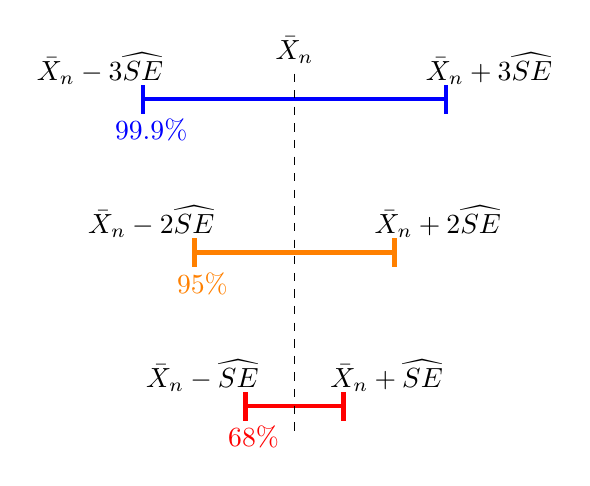
\begin{tikzpicture}[scale = 0.65]
	\draw [ultra thick, blue, |-|](-3,3) -- (3,3);
	\node [above] at (-3.8,3.1) {$\bar{X}_n-3 \widehat{SE}$};
	\node [above] at (3.8,3.1) {$\bar{X}_n+3  \widehat{SE}$};
	\node [below, blue] at (-2.8, 2.8) {99.9\%};	
	
	\draw [ultra thick, orange, |-|](-2,0) -- (2,0);
	\node [above] at (-2.8,0.1) {$\bar{X}_n-2 \widehat{SE}$};
	\node [above] at (2.8,0.1) {$\bar{X}_n+2 \widehat{SE}$};
	\node [below, orange] at (-1.8, -0.2) {95\%};	

	\draw [ultra thick, red, |-|](-1,-3) -- (1,-3);
	\node [above] at (-1.8,-2.9) {$\bar{X}_n -  \widehat{SE}$};
	\node [above] at (1.8,-2.9) {$\bar{X}_n +  \widehat{SE}$};
	\node [below, red] at (-0.8, -3.2) {68\%};	
	
	\draw [dashed](0,3.5) -- (0,-3.5);
	\node [above] at (0,3.5) {$\bar{X}_n$};	
\end{tikzpicture}
\singlespacing
\caption{\small  Each CI gives a range of ``plausible'' values for the population mean $\mu$, centered at the sample mean $\bar{X}_n$. Values near the middle are ``more plausible'' in the sense that a small reduction in confidence level gives a much shorter interval centered in the same place. This is because the sample mean is unlikely to take on values far from the population mean in repeated sampling (CLT).}
\end{figure}

\end{frame}
%%%%%%%%%%%%%%%%%%%%%%%%%%%%%%%%%%%%%%%%
\begin{frame}
\frametitle{CI for Difference of Population Means Using CLT}

\begin{block}{Previous Example}
Used CLT to get CI for difference of population proportions based on independent samples.
\end{block}

\begin{block}{But Proportions are a Kind of Mean!}
Population proportion is mean of Bernoulli random variable, and sample proportion is mean of sample comprised of ones and zeros.
\end{block}

\vspace{2em}

\alert{The general problem of constructing a CI for the difference of population means using the CLT is essentially identical to what we did last time for population proportions.}

\end{frame}

%%%%%%%%%%%%%%%%%%%%%%%%%%%%%%%%%%%%%%%%
\begin{frame}
\frametitle{CI for Difference of Population Means Using CLT}
\begin{block}{Setup: Independent Random Samples}
$X_1, \hdots, X_n \sim \mbox{iid}$ with mean $\mu_X$ and variance $\sigma_X^2$\\ $Y_1, \hdots, Y_m \sim \mbox{iid}$ with mean $\mu_Y$ and variance $\sigma_Y^2$\\
\emph{where each sample is independent of the other } 
\end{block}

\begin{alertblock}{We Do Not Assume the Populations are Normal!}
\end{alertblock}

\end{frame}



%%%%%%%%%%%%%%%%%%%%%%%%%%%%%%%%%%%%%%%%
\begin{frame}
\frametitle{Difference of Sample Means $\bar{X}_n-\bar{Y}_m$ and the CLT}
\begin{block}{What We Have}
Approx.\ sampling dist.\ for \emph{individual}  sample means from CLT:
\alert{$\bar{X}_n\approx N\left(\mu_X, \widehat{SE}(\bar{X}_n)^2\right), \quad \bar{Y}_m\approx N\left(\mu_Y, \widehat{SE}(\bar{Y}_m)^2\right)$}
\end{block}

\begin{block}{What We Want}
Sampling Distribution of the \emph{difference} $\bar{X}_n - \bar{Y}_m$
\end{block}

\begin{block}{Use Independence of the Two Samples}
\alert{$\bar{X}_n - \bar{Y}_m\approx N\left( \mu_X - \mu_Y, \widehat{SE}(\bar{X}_n)^2 +\widehat{SE}(\bar{Y}_m)^2\right)$}



$$\implies \widehat{SE}(\bar{X}_n - \bar{Y}_m) =  \sqrt{\widehat{SE}(\bar{X}_n)^2 +\widehat{SE}(\bar{Y}_m)^2}  = \sqrt{\displaystyle\frac{S_x^2}{n} + \frac{S_y^2}{m} }$$
\end{block}

\end{frame}
%%%%%%%%%%%%%%%%%%%%%%%%%%%%%%%%%%%%%%%%
\begin{frame}
\frametitle{CI for Difference of Pop.\ Means (Independent Samples)}

$X_1, \hdots, X_n \sim \mbox{iid}$ with mean $\mu_X$ and variance $\sigma_X^2$\\ $Y_1, \hdots, Y_m \sim \mbox{iid}$ with mean $\mu_Y$ and variance $\sigma_Y^2$\\
\emph{where each sample is independent of the other } 


	$$\left(\bar{X}_n - \bar{Y}_m\right) \pm \texttt{qnorm}(1-\alpha/2) \sqrt{\frac{S_x^2}{n} + \frac{S_y^2}{m}}$$
	\alert{Approximation based on the CLT. Works well provided $n,m$ large.}
\end{frame}
%%%%%%%%%%%%%%%%%%%%%%%%%%%%%%%%%%%%%%%%

\begin{frame}
\frametitle{The Anchoring Experiment}
At the beginning of the last semester, students were each shown a ``random number.'' In fact the numbers weren't random: there was a ``Hi'' group that was shown 65 and a ``Lo'' group that was shown 10. The students were randomly assigned to one of these two groups and shown their ``random'' number. Then they were asked what proportion of UN member states are located in Africa.  Let's take a look at the results...


\end{frame}

%\begin{frame}
%\frametitle{Boxplot of Anchoring Experiment}
%\begin{figure}
%\centering
%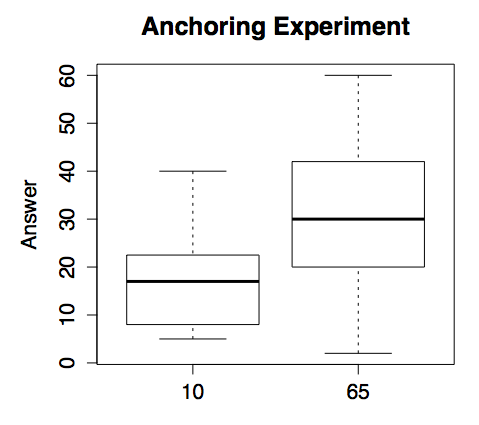
\includegraphics[scale=0.4]{./images/anchor_experiment}
%\end{figure}
%\end{frame}


\begin{frame}
\frametitle{Anchoring Experiment}
\small
\singlespacing
%\begin{block}{From what population is the sample drawn?} 
%US College Students? Penn Students? Penn Econ Majors? 
%\end{block}

\begin{block}{Do We Have a Random Sample?} 
Definitely not a random sample of US College Students. Possibly a random sample of Penn Econ Majors since Econ 103 is required. 
\end{block}


%\begin{block}{Observational or Experimental Data?} 
%Randomized Experiment drew from a bag of ``random'' numbers 
%\end{block}

\begin{block}{Are the two samples independent?}
Yes: Students were told not to show their number to any other students or consult with them in any way. 
\end{block}

\begin{block}{What is the Research Question?} 
Does ``anchoring'' cause of bias in decision-making? 
\end{block}
\end{frame}
%%%%%%%%%%%%%%%%%%%%%%%%%%%%%%%%%%%%%%%%
\begin{frame}[t]
\frametitle{Past Semester's Anchoring Experiment}

\begin{columns}
	\column{0.4\textwidth}
	\begin{figure}
	\centering
	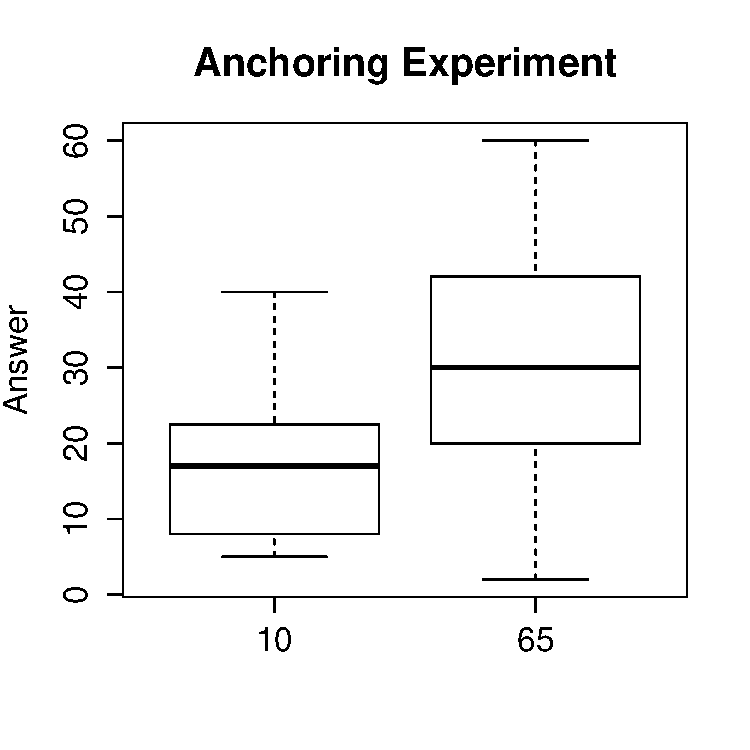
\includegraphics[scale = 0.4]{./images/anchoring_boxplot}
	\end{figure}

	\column{0.5\textwidth}
	\begin{block}{``Lo'' Group -- Shown 10 }
	$m_{Lo} = 43$\\ $\bar{y}_{Lo} = 17.1$ \\ $s^2_{Lo} = 86$
\end{block}
		\begin{block}{``Hi'' Group -- Shown 65 }
		$n_{Hi} =46$\\ $\bar{x}_{Hi} = 30.7$\\ $s^2_{Hi} = 253$
\end{block}

\end{columns}
\end{frame}
%%%%%%%%%%%%%%%%%%%%%%%%%%%%%%%%%%%%%%%%
\begin{frame}
\frametitle{ME for approx.\ 95\% for Difference of Means}

\small
\singlespacing
\begin{columns} 
	\column{0.5\textwidth}
	\begin{block}{``Lo'' Group}
		\begin{eqnarray*}
			\bar{y}_{Lo} &=&17.1 \\
			m_{Lo} &=& 43\\  
			s^2_{Lo} &=& 86\\ 
			\widehat{SE}(\bar{y}_{Lo})^2 &=& \frac{s^2_{Lo}}{m_{Lo}} = 2
		\end{eqnarray*}
	\end{block}
	
	\column{0.5\textwidth}
		\begin{block}{``Hi'' Group}
		\begin{eqnarray*}
			\bar{x}_{Hi} &=& 30.7\\
			n_{Hi} &=& 46\\  
			s^2_{Hi} &=& 253\\
			\widehat{SE}(\bar{x}_{Hi})^2 &=& \frac{s^2_{Hi}}{n_{Hi}} = 5.5
		\end{eqnarray*}
	\end{block}
\end{columns}

\pause
	\begin{eqnarray*}
		\bar{X}_{Hi} - \bar{Y}_{Lo} &=& 30.7 - 17.1 =  13.6\\ \pause
		\widehat{SE}(\bar{X}_{Hi} - \bar{Y}_{Lo}) &=& \pause \sqrt{\widehat{SE}(\bar{X}_{Hi})^2 + \widehat{SE}(\bar{Y}_{Lo})^2} = \sqrt{7.5}  \approx 2.7 \pause \Rightarrow ME \approx 5.4 \pause 
	\end{eqnarray*}
	$$\alert{\boxed{\mbox{Approximate 95\% CI} \quad (8.2, 19)}} \quad \mbox{What can we conclude?}$$


\end{frame}

\begin{frame}
\frametitle{Which is the Harder Exam?}
Last fall Econ 103 had two midterms. Here are the scores:
% latex.default(round(grades.out, 1), file = "grades.tex", rowname = NULL) 
%
\begin{table}[!tbp]
\begin{center}
\begin{tabular}{rrrr}
\hline\hline
\multicolumn{1}{r}{Student}&\multicolumn{1}{r}{Exam 1}&\multicolumn{1}{r}{Exam 2}&\multicolumn{1}{r}{Difference}\tabularnewline
\hline
$ 1$&$57.1$&$60.7$&$  3.6$\tabularnewline
$ 2$&$77.1$&$77.9$&$  0.7$\tabularnewline
$ 3$&$83.6$&$93.6$&$ 10.0$\tabularnewline
\vdots&\vdots&\vdots&\vdots\\
$69$&$75.0$&$74.3$&$ -0.7$\tabularnewline
$70$&$96.4$&$86.4$&$-10.0$\tabularnewline
$71$&$78.6$&$82.9$&$  4.3$\tabularnewline
\hline
Sample Mean: & 79.6 & 81.4  &1.8\\
\hline
\end{tabular}
\end{center}
\end{table}

\alert{Was the second exam easier than the first?}
\end{frame}
%%%%%%%%%%%%%%%%%%%%%%%%%%%%%%%%%%%%%%%%
\begin{frame}
\frametitle{What is the population model?}

\begin{block}{What does it mean to say that one exam is easier?} 
	\begin{itemize}
	\item Exam partly measures what you know and is partly random 
		\begin{itemize}
			\item You could have a bad day
			\item The exam might focus on your weaker areas
		\end{itemize}
	\item If a very large number of students take the exams, the randomness should \emph{average out}.
		\item If a small number of students take the exams, they might score lower on the ``easier exam'' because of bad luck.
	\end{itemize}
\end{block}




 \end{frame}


%%%%%%%%%%%%%%%%%%%%%%%%%%%%%%%%%%%%%%%%
\begin{frame}
\frametitle{Are the two samples independent? \hfill 
\includegraphics[scale = 0.05]{./images/clicker}}
Suppose we treat the scores on the first midterm as one sample and the scores on the second as another. Are these samples independent?

\begin{enumerate}[(a)]
	\item Yes
	\item No
	\item Not Sure
\end{enumerate}

\pause
\alert{No -- Each sample contains exactly the same students!}

\end{frame}
%%%%%%%%%%%%%%%%%%%%%%%%%%%%%%%%%%%%%%%%
\begin{frame}
\frametitle{Dependent Samples -- Same Students Took Each Exam}
% latex.default(round(grades.out, 1), file = "grades.tex", rowname = NULL) 
%
\begin{table}[!tbp]
\begin{center}
\begin{tabular}{rccr}
\hline\hline
\multicolumn{1}{r}{Student}&\multicolumn{1}{c}{Exam 1}&\multicolumn{1}{c}{Exam 2}&\multicolumn{1}{r}{Difference}\tabularnewline
\hline
$ 1$&$57.1$&$60.7$&$  3.6$\tabularnewline
\vdots&\vdots&\vdots&\vdots\\
$71$&$78.6$&$82.9$&$  4.3$\tabularnewline
\hline
Sample Mean: & 79.6 & 81.4  &1.8\\
%Sample Var. &117  & 151 & 124\\
\alert{Sample Corr.} & \multicolumn{2}{c}{\alert{0.54}}&\\
\hline
\end{tabular}
\caption{The samples are dependent because each includes \emph{exactly the same students}. Indeed, we see that scores on the two exams are strongly positively correlated: students who did well on the first exam tended to do well on the second.}
\end{center}
\end{table}

\end{frame}
%%%%%%%%%%%%%%%%%%%%%%%%%%%%%%%%%%%%%%%%
\begin{frame}
\frametitle{What's going on here?}

We don't really have two samples: we have a \emph{single} sample of students, each of whom took two exams. This is really a \emph{one sample problem} based on the \emph{difference of individual exam scores}. Such a setup is sometimes referred to as \alert{matched pairs data}

\vspace{2em}

\fbox{Let $D_i = X_i - Y_i$ be the difference of student $i$'s exam scores.}

\end{frame}
%%%%%%%%%%%%%%%%%%%%%%%%%%%%%%%%%%%%%%%%
\begin{frame}
\frametitle{Solving this as a One-Sample Problem}
\small
\fbox{Let $D_i = X_i - Y_i$ be the difference of student $i$'s exam scores.}

\vspace{2em}
I calculated the following in R:
	\begin{eqnarray*}
	\bar{D}_n &=& \frac{1}{n}\sum_{i=1}^n D_i \approx 1 .8\\
	S^2_D &=& \frac{1}{n-1}\sum_{i=1}^n (D_i - \bar{D})^2 \approx 	124\\ 
	\widehat{SE}(\bar{D}_n) &=&(S_D /\sqrt{n}) \approx \sqrt{124/71} \approx 1.3 
	\end{eqnarray*}
	
\vspace{1em}
\alert{Approximate 95\% CI Based on the CLT:}
$$\alert{\boxed{1.8 \pm 2.6 = (-0.8, 4.4)}} \quad \mbox{What is our conclusion?}$$

\end{frame}
%%%%%%%%%%%%%%%%%%%%%%%%%%%%%%%%%%%%%%%%
\begin{frame}
	\begin{center}
	\Huge How are the Independent Samples and Matched Pairs Problems Related?
	\end{center}
\end{frame}

%%%%%%%%%%%%%%%%%%%%%%%%%%%%%%%%%%%%%%%%
\begin{frame}
\frametitle{Difference of Means = Mean of Differences?\hfill 
\includegraphics[scale = 0.05]{./images/clicker}}
\fbox{Let $D_i = X_i - Y_i$ be the difference of student $i$'s exam scores.}

True or False:
	$$\bar{D}_n = \bar{X}_n - \bar{Y}_n$$

\begin{enumerate}[(a)]
	\item True
	\item False
	\item Not Sure
\end{enumerate}

\end{frame}
%%%%%%%%%%%%%%%%%%%%%%%%%%%%%%%%%%%%%%%%
\begin{frame}
\frametitle{Difference of Means Equals Mean of Differences}
\fbox{Let $D_i = X_i - Y_i$ be the difference of student $i$'s exam scores.}

\vspace{1em}
\alert{Sample mean of differences \emph{equals} difference of sample means}
\begin{eqnarray*}
	\bar{D}_n &=& \frac{1}{n}\sum_{i=1}^n D_i = \frac{1}{n}\sum_{i=1}^n (X_i - Y_i)\\
	& =& \left(\frac{1}{n}\sum_{i=1}^n X_i \right)- \left(\frac{1}{n}\sum_{i=1}^n Y_i \right)= \bar{X}_n - \bar{Y}_n
\end{eqnarray*}



\vspace{2em}

\alert{Linearity of Expectation holds even under dependence:}
\begin{eqnarray*}
	E[\bar{D}_n] = E[\bar{X}_n - \bar{Y}_n] = E[\bar{X}_n] - E[\bar{Y}_n] = \mu_X - \mu_Y
\end{eqnarray*}


\end{frame}

%%%%%%%%%%%%%%%%%%%%%%%%%%%%%%%%%%%%%%%%
\begin{frame}
\frametitle{Exam Dataset}
% latex.default(round(grades.out, 1), file = "grades.tex", rowname = NULL) 
%
\begin{table}[!tbp]
\begin{center}
\begin{tabular}{rccr}
\hline\hline
\multicolumn{1}{r}{Student}&\multicolumn{1}{c}{Exam 1}&\multicolumn{1}{c}{Exam 2}&\multicolumn{1}{r}{Difference}\tabularnewline
\hline
$ 1$&$57.1$&$60.7$&$  3.6$\tabularnewline
\vdots&\vdots&\vdots&\vdots\\
$71$&$78.6$&$82.9$&$  4.3$\tabularnewline
\hline
Sample Mean: & 79.6 & 81.4  &1.8\\
\hline
\end{tabular}
\end{center}
\end{table}


\begin{eqnarray*}
	\bar{D}_n &=& 1.8\\ 
	\bar{X}_n - \bar{Y}_n &=&  81.4 - 79.6 =   1.8  \;\alert{\checkmark}
\end{eqnarray*}

\end{frame}

%%%%%%%%%%%%%%%%%%%%%%%%%%%%%%%%%%%%%%%%

\begin{frame}
\frametitle{...But Dependence Changes the Variance Calculation}
\small
Recall that for any two RVs $X,Y$ and constants $a,b$
$$Var(aX + bY) = a^2 Var(X) + b^2Var(Y) + 2ab Cov(X,Y)$$

\pause
From the last slide, $\bar{D}_n = \bar{X}_n - \bar{Y}_n$, hence
\begin{eqnarray*}
Var(\bar{D}_n) &=& Var(\bar{X}_n - \bar{Y}_n)\\ \pause
 &=& Var(\bar{X}_n) + Var(\bar{Y}_n) - 2Cov(\bar{X}_n, \bar{Y}_n)\\ \pause
	&=& \frac{\sigma_X^2}{n} + \frac{\sigma_Y^2}{n} - 2Cov(\bar{X}_n, \bar{Y}_n) \alert{\neq \frac{\sigma_X^2}{n} + \frac{\sigma_Y^2}{n}}\\
\end{eqnarray*}


\alert{Since the samples are correlated, $Cov(\bar{X}_n, \bar{Y}_n)\neq 0$! Hence the standard error estimate for independent samples, $\sqrt{S^2_X/n + S^2_Y/n}$, is  inappropriate!}


\end{frame}
%%%%%%%%%%%%%%%%%%%%%%%%%%%%%%%%%%%%%%%%

\begin{frame}
\frametitle{Another Way to Calculate Sample Var.\ of the Differences}
\footnotesize
Variance of the differences can also be calculated from the sample variance for each exam along with the correlation between them:
\begin{eqnarray*}
	S_D^2&=& \frac{1}{n-1}\sum_{i=1}^n \left( D_i - \bar{D}_n\right)^2 = \pause \frac{1}{n-1}\sum_{i=1}^n \left[ \left( X_i - Y_i\right) - \left( \bar{X}_n - \bar{Y}_n\right)\right]^2\\ \pause
	&=&\frac{1}{n-1}\sum_{i=1}^n \left[ \left( X_i - \bar{X}_n\right) - \left( Y_i - \bar{Y}_n\right)\right]^2\\ \pause
	&=&\frac{1}{n-1}\sum_{i=1}^n \left[ \left( X_i - \bar{X}_n\right)^2 + \left( Y_i - \bar{Y}_n\right)^2 - 2\left(X_i - \bar{X}_n\right)\left(Y_i - \bar{Y}_n\right)\right]\\ \pause
	&=& S_X^2 + S_Y^2 - 2 S_{XY}\\ \pause
	&=& S_X^2 + S_Y^2 - 2 S_X S_Y r_{XY}
\end{eqnarray*}

\vspace{1em}
\alert{$\boxed{r_{XY} > 0 \implies S_D^2 < S_X^2 + S_Y^2}$}

\end{frame}
%%%%%%%%%%%%%%%%%%%%%%%%%%%%%%%%%%%%%%%%
\begin{frame}
\frametitle{Dependent Samples -- Calculating the ME}
% latex.default(round(grades.out, 1), file = "grades.tex", rowname = NULL) 
%
\begin{table}[!tbp]
\begin{center}
\begin{tabular}{rccr}
\hline\hline
\multicolumn{1}{r}{Student}&\multicolumn{1}{c}{Exam 1}&\multicolumn{1}{c}{Exam 2}&\multicolumn{1}{r}{Difference}\tabularnewline
\hline
$ 1$&$57.1$&$60.7$&$  3.6$\tabularnewline
\vdots&\vdots&\vdots&\vdots\\
$71$&$78.6$&$82.9$&$  4.3$\tabularnewline
\hline
Sample Var. &117  & 151 & \alert{\fbox{?}}\\
Sample Corr.& \multicolumn{2}{c}{0.54}&\\
\hline
\end{tabular}
\end{center}
\end{table}

$$117 + 151 - 2 \times 0.54 \times \sqrt{117 \times 151} \approx 124   \;\alert{\checkmark}$$

%\alert{This agrees with what we got when we did calculations directly for the differences!}
\end{frame}
%%%%%%%%%%%%%%%%%%%%%%%%%%%%%%%%%%%%%%%%
\begin{frame}
\frametitle{The ``Wrong CI'' (Assuming Independence) is Too Wide}
\footnotesize
% latex.default(round(grades.out, 1), file = "grades.tex", rowname = NULL) 
%
\begin{table}[!tbp]
\begin{center}
\begin{tabular}{rccr}
\hline\hline
\multicolumn{1}{r}{Student}&\multicolumn{1}{c}{Exam 1}&\multicolumn{1}{c}{Exam 2}&\multicolumn{1}{r}{Difference}\tabularnewline
\hline
Sample Size & 71 & 71 & 71\\
Sample Mean & 79.6 & 81.4  &1.8\\
Sample Var. &117  & 151 & 124\\
Sample Corr.& \multicolumn{2}{c}{0.54}&\\
\hline
\end{tabular}
\end{center}
\end{table}

\singlespacing
\small

\begin{block}{Wrong Interval -- Assumes Independence}
$$1.8 \pm 2\times  \sqrt{117/71 + 151/71} \implies (-2.1, 5.7)$$
\end{block}

\pause

\begin{block}{Correct Interval -- Matched Pairs}
$$1.8 \pm 2\times  \sqrt{124/71} \implies (-0.8, 4.4)$$
\end{block}

\pause
\alert{Top CI is too wide because the exam scores are positively correlated, so the variance of the differences is less than the sum of the variances of the two exams. Both CIs, however, are correctly centered.}

\end{frame}
%%%%%%%%%%%%%%%%%%%%%%%%%%%%%%%%%%%%%%%%


\begin{frame}
\frametitle{Overview: Independent Samples Versus Matched Pairs}

\begin{itemize}
	\item When you see a problem that involves two datasets, think carefully about whether they should be treated as independent samples or if they're really matched pairs. The CIs differ! 
	\item The matched pairs calculations can be done in two ways: 
		\begin{enumerate}
			\item Direct calculation using the sample mean and standard deviation of the individual differences $D_i = X_i - Y_i$ 
			\item Indirect calculation using the sample mean and standard deviation of the X's and Y's \emph{separately} along with the sample correlation between them. 
		\end{enumerate}
\end{itemize}
\end{frame}


%%%%%%%%%%%%%%%%%%%%%%%%%%%%%%%%%%%%%%%%
%\begin{frame}
%\begin{center}
	%\huge Refined 95\% CI for Proportion: \\``Add Two Successes and Failures''
%\end{center}
%\end{frame}
%%%%%%%%%%%%%%%%%%%%%%%%%%%%%%%%%%%%%%%%
%\begin{frame}
%\frametitle{Refined 95\% CI for Population Proportion}
%\small
%\alert{\fbox{Add four ``fake'' observations to the dataset: two zeros and two ones.}}
%\vspace{1em}

%\begin{columns}

%\column{0.5\textwidth}
%\begin{block}{Textbook Confidence Interval}
%$$\widehat{p} = \frac{1}{n}\left(\sum_{i=1}^n X_i\right)$$

%$$\widehat{p}\pm \texttt{qnorm}\left(0.975\right) \times\sqrt{\frac{\widehat{p}(1-\widehat{p})}{n}}$$
%\end{block}

%\column{0.5\textwidth}
%\begin{block}{Refined Confidence Interval}
%$$\alert{\widetilde{p}} = \frac{1}{n+\alert{4}} \left(\alert{2}+ \sum_{i=1}^n X_i\right)$$

%$$\alert{\widetilde{p}} \pm \texttt{qnorm}\left(0.975\right) \times \sqrt{\frac{\alert{\widetilde{p}}(1-\alert{\widetilde{p}})}{n+\alert{4}}}$$

%\end{block}

%\end{columns}

%\vspace{1em}

%\alert{This is related to problem 7-13 in the textbook...}
%\end{frame}
%%%%%%%%%%%%%%%%%%%%%%%%%%%%%%%%%%%%%%%%
%\begin{frame}
%\frametitle{Refined 95\% CI for Difference of Population Proportions}
%\small
%\alert{\fbox{Add four ``fake'' observations total: two to \emph{each} dataset (a one and a zero).}}

%\begin{block}{Textbook Confidence Interval}
%$$\widehat{p} - \widehat{q} = \frac{1}{n}\left(\sum_{i=1}^n X_i\right) - \frac{1}{m}\left(\sum_{i=1}^n Y_i\right)$$

%	$$\left(\widehat{p} -\widehat{q}\right)\pm \texttt{qnorm}(0.975) \times \sqrt{\frac{\widehat{p}(1-\widehat{p})}{n} + \frac{\widehat{q}(1-\widehat{q})}{m}}$$

%\end{block}


%\begin{block}{Refined Confidence Interval}
	%$$\alert{p^*} - \alert{q^*} = \frac{1}{n+\alert{2}}\left(1 + \sum_{i=1}^n X_i\right) - \frac{1}{m+\alert{2}}\left(1 + \sum_{i=1}^m Y_i\right) $$

%	$$\left(\alert{p^*} -\alert{q^*}\right)\pm \texttt{qnorm}(0.975) \times \sqrt{\frac{\alert{p^*}(1-\alert{p^*})}{n+\alert{2}} + \frac{\alert{q^*}(1-\alert{q^*})}{m+\alert{2}}}$$
%\end{block}

%\end{frame}
%%%%%%%%%%%%%%%%%%%%%%%%%%%%%%%%%%%%%%%%
%\begin{frame}
%\frametitle{What is the point of this?}

%\begin{block}{Recall from Last Time}
%Our CIs for proportions are \emph{approximations} based on the CLT. 
%\end{block}

%\begin{block}{When is the approximation good?} 
%Large sample size (n,m) and true population proportions (p,q) that aren't too close to zero or one. 
%\end{block}


%\begin{alertblock}{Why the Refined Intervals?}
%They work well even when sample sizes ($n,m$) are small and true population proportions ($p,q$) are close to zero or one. When the samples are large, the refined intervals are practically identical to the textbook intervals. 
%\end{alertblock}
%\end{frame}
%%%%%%%%%%%%%%%%%%%%%%%%%%%%%%%%%%%%%%%%
\begin{frame}
	\frametitle{Confidence Intervals We've Covered}
	\begin{enumerate}
		\item Exact CIs based on assumption of Normality:
			\begin{enumerate}[(a)]
				\item CI for population mean, population variance known (\texttt{qnorm})
				\item CI for population mean, population variance unknown (\texttt{qt})
				\item CI for population variance (\texttt{qhisq})
				\item CI for difference of population means, indep.\ samples (\texttt{qt})
			\end{enumerate}
			\vspace{0.1in}
		\item Approximate CIs using CLT (\texttt{qnorm})
			\begin{enumerate}[(a)]
				\item CI for population mean (also matched pairs data)
				\item CI for difference of population means, independent samples
				\item CIs for proportions and differences of proportions 
		%			\begin{enumerate}[(i)]
			%			\item ``Textbook'' version -- use sample proportions
				%		\item ``Refined'' version -- ``add two successes and failures (total)''			
				%	\end{enumerate}
			\end{enumerate}
	\end{enumerate}
  \alert{In nearly all real applications we'll use 2, but you need to understand what's going on in 1 as well.}
\end{frame}
%%%%%%%%%%%%%%%%%%%%%%%%%%%%%%%%%%%%%%%%


\end{document}
